\documentclass[unicode, 14pt, aspectratio=169]{beamer}
\usepackage{bussproofs}
\usetheme{titech}
\addbibresource{main.bib}
 \date{\number\year 年\number\month 月\number\day 日}
\title{型理論のはじまり}
\author{\texttt{ryotaro612}}

\newcommand\blfootnote[1]{%
  \begingroup
  \renewcommand\thefootnote{}\footnote{#1}%
  \addtocounter{footnote}{-1}%
  \endgroup
}

\begin{document}
\begin{frame}[noframenumbering, plain]
\titlepage
\end{frame}
\section{導入}
\begin{frame}
  \frametitle{資料の目的}
  {\large 型理論に関わる分野の紹介}
  \par
  \vspace{16pt}
  参考資料に関わる分野
  \begin{itemize}
  \item 論理学
  \item 集合論
  \item 記号論
  \item 構造主義
  \item 哲学、とくに分析哲学
  \end{itemize}
\end{frame}
\section{幾何学}
\begin{frame}
  \frametitle{ギリシアで発展した幾何学}
  {\large 幾何学の知識は\textcolor{highlight}{証明}\footnote{作図を証明とすることもあった。ギリシア語の「証明する」という単語(デイクニュミ)には「図示する」という意味もある。demostrationの語源}された定理の集積}
\begin{columns}
  \begin{column}{0.25\textwidth}
    \begin{center}
      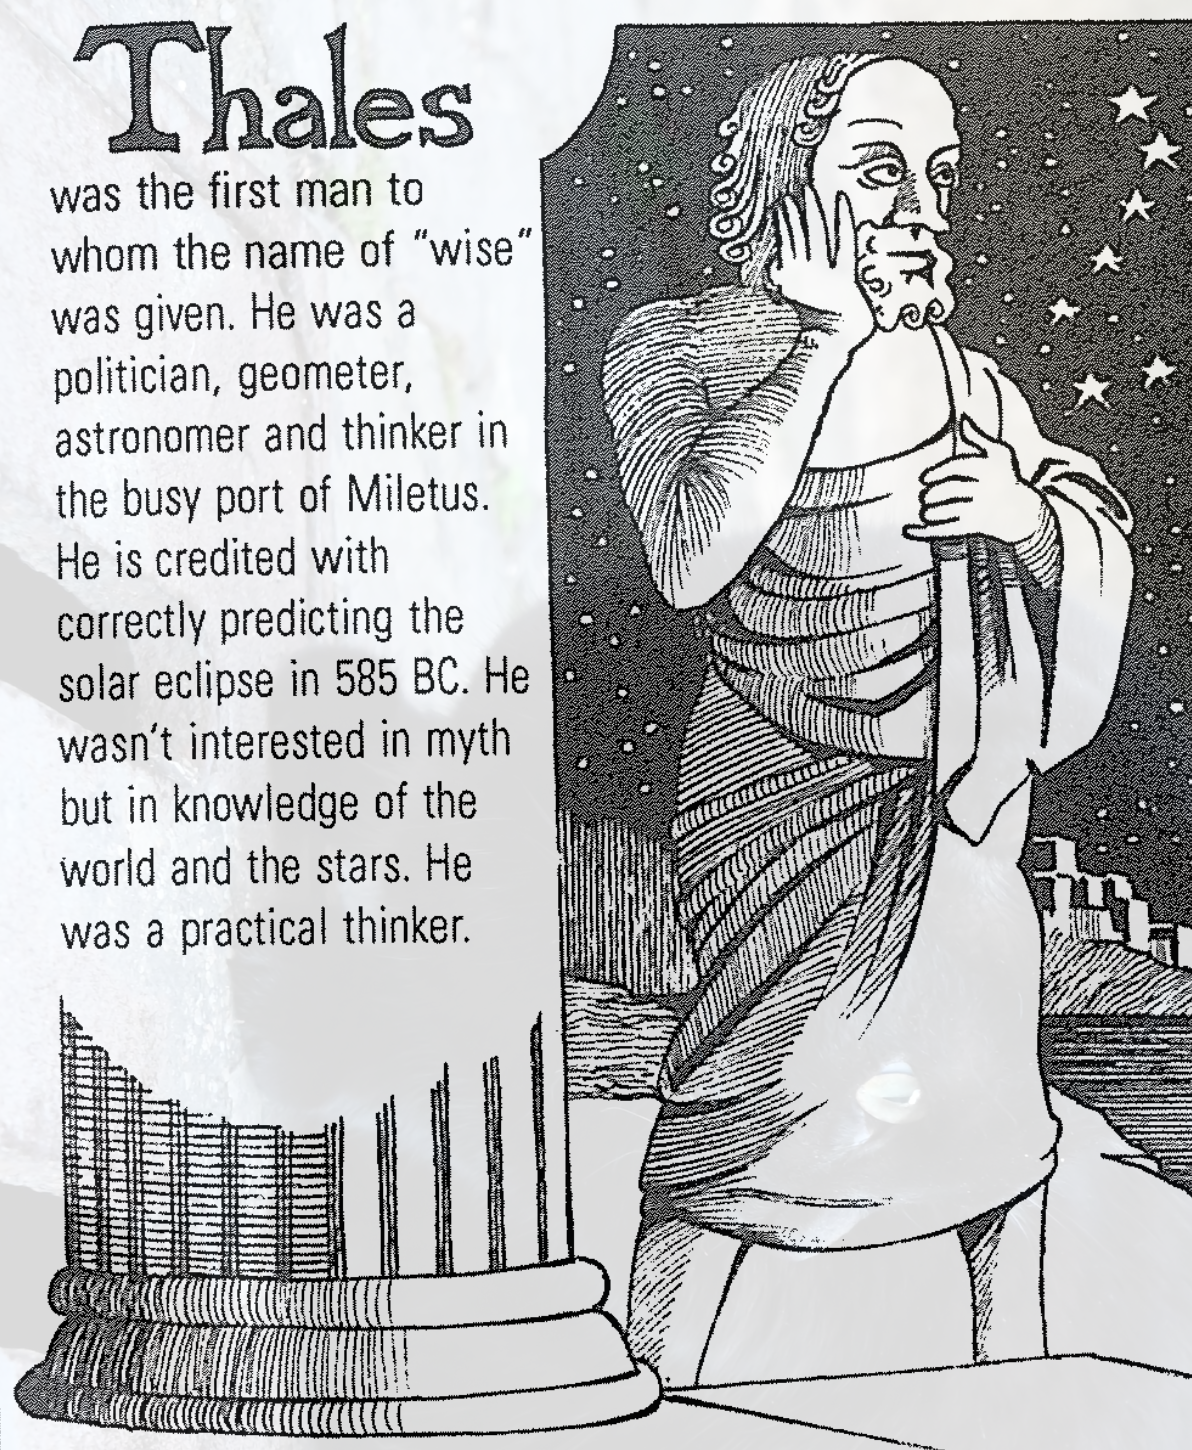
\includegraphics[width=0.7\textwidth]{images/thales.png}
    \end{center}
  \end{column}
  \begin{column}{0.25\textwidth}
    \begin{center}
      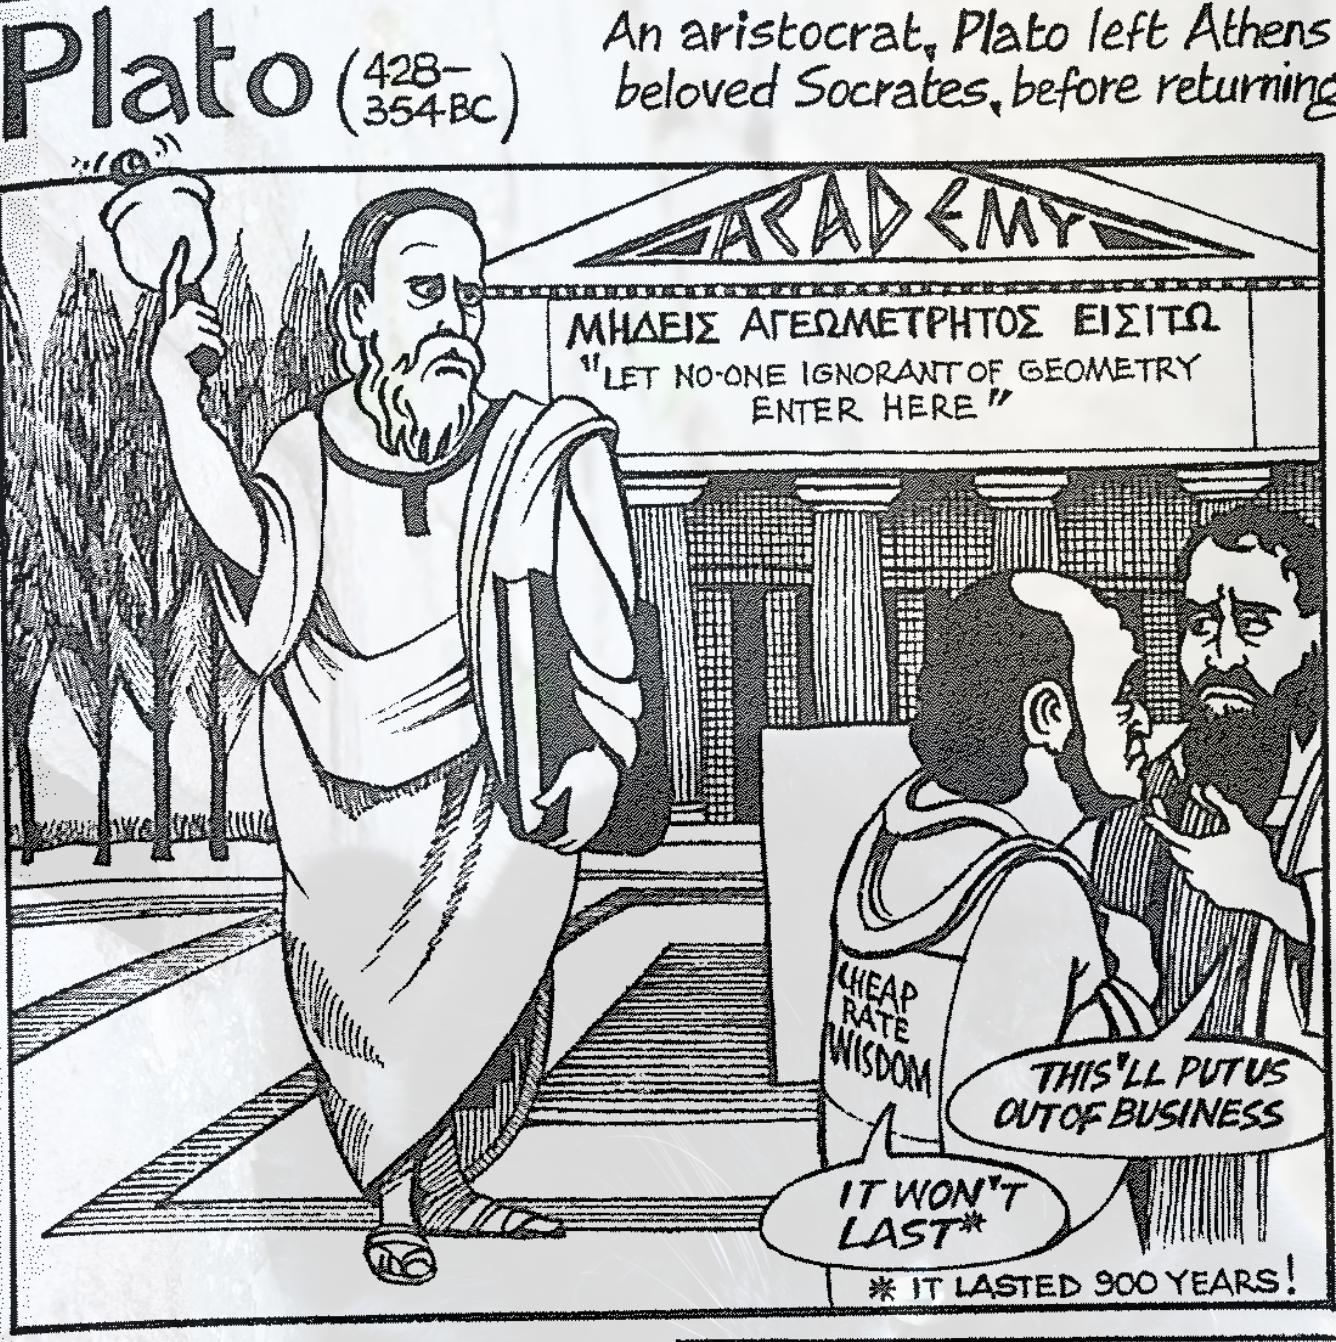
\includegraphics[width=0.7\textwidth]{images/plato.png}
    \end{center}
  \end{column}
  \begin{column}{0.25\textwidth}
    \begin{center}
      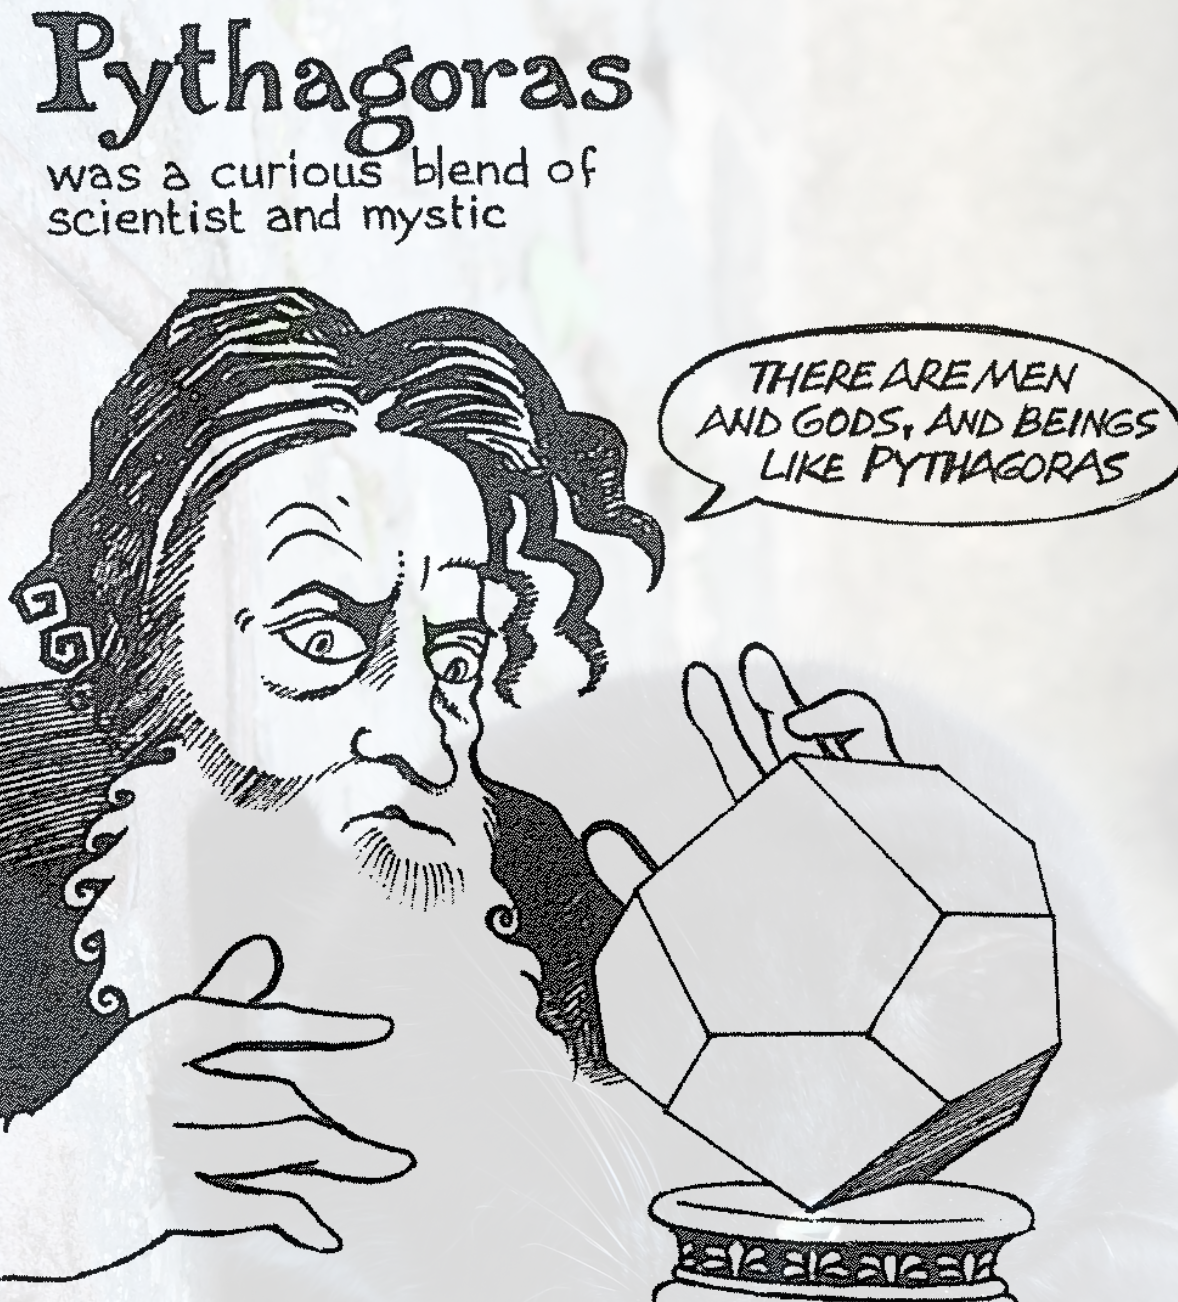
\includegraphics[width=0.7\textwidth]{images/pythagoras.png}
    \end{center}
  \end{column}
  \begin{column}{0.25\textwidth}
    \begin{center}
      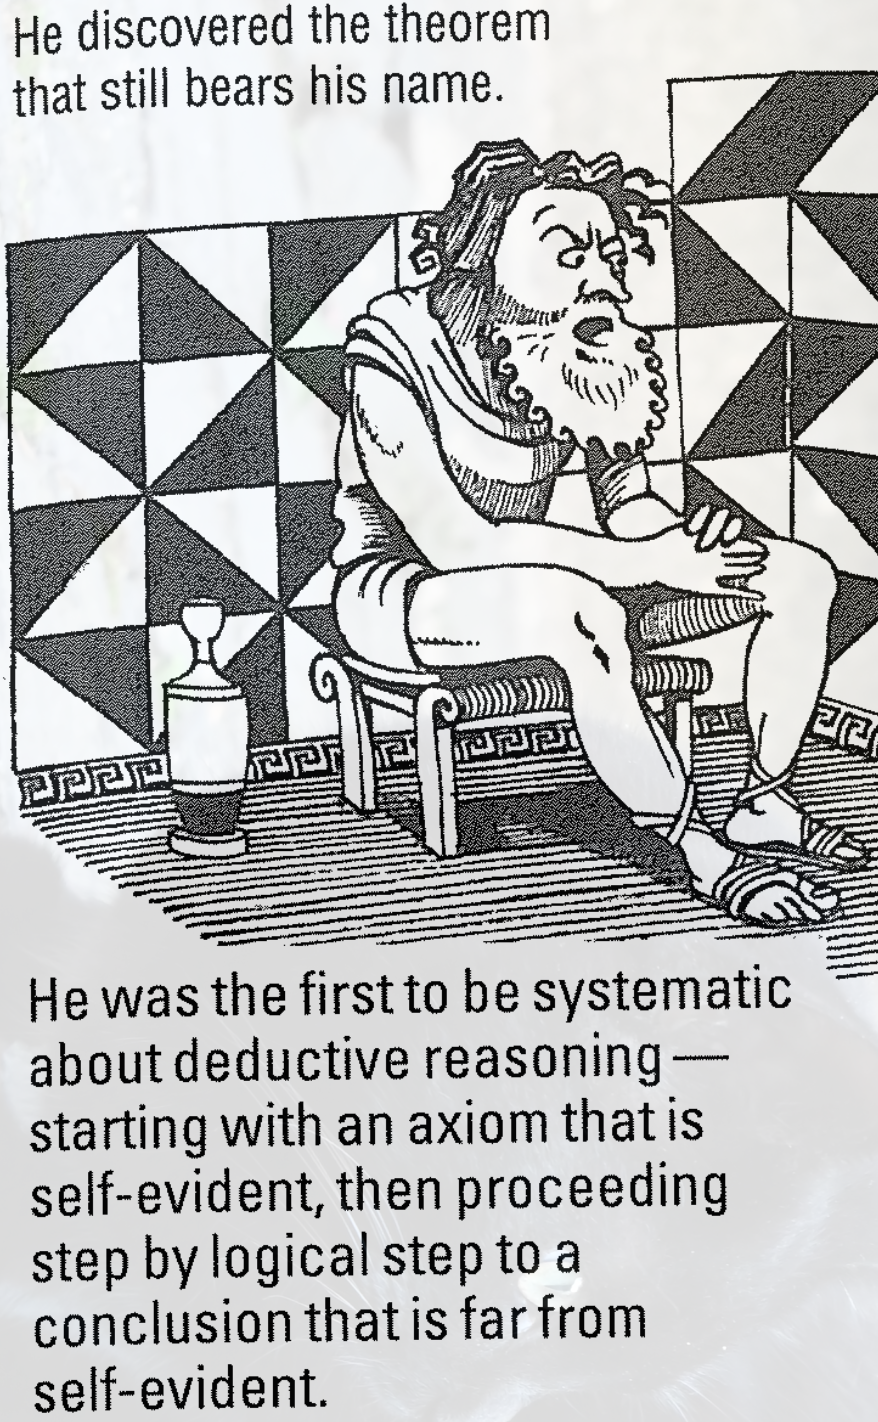
\includegraphics[width=0.7\textwidth]{images/pythagoras2.png}
    \end{center}
  \end{column}  
\end{columns}
\blfootnote{図はPhilosophy for beginners\supercite{philosophy-for-begginers}より} 
\end{frame}
\begin{frame}
  \frametitle{ユークリッドの原論}
  {\large 幾何学が定義、公理、公準\footnote{公理は量などの一般対象の前提、公準は幾何学の対象の前提}、命題、証明に整理された}
  \par
  \vspace{16pt}
  具体例
  \begin{description}
  \item[定義1] 点とは部分をもたないもの
  \item[定義2] 線は幅のない長さ
  \item[定義3] 面は長さと幅だけをもつもの
  \item[公理5] \textcolor{highlight}{全体は部分より大きい}
  \item[命題5] 二等辺三角形の底辺はたがいに等しい
  \end{description}
\end{frame}
\begin{frame}
  \frametitle{5つの公準}
  {\large 5番目の公準は複雑}
  \par
  \vspace{16pt}  
  \begin{enumerate}
  \item 任意の点から任意の点に直線を引くこと
  \item 有限な線分を連続して直線に延長すること
  \item 任意の点と半径で円を描くこと
  \item すべての直角は等しいこと
  \item \textcolor{highlight}{二直線が一直線と交わるとき、同じ側にできる内角の和が\\二直角よりも小さいなら二直線はその側に延長すると交わる}
  \end{enumerate}
\end{frame}
\begin{frame}[t]
  \frametitle{公準5の別名は平行線公理}
  {\large 公準5を換言すると任意の直線と直線外の任意の一点があるとき一点を通り\textcolor{highlight}{直線に平行な直線は1本}だけ}
  \blfootnote{図は『数学の世界史』\supercite{suugaku-no-sekaishi}より}
  \begin{figure}
    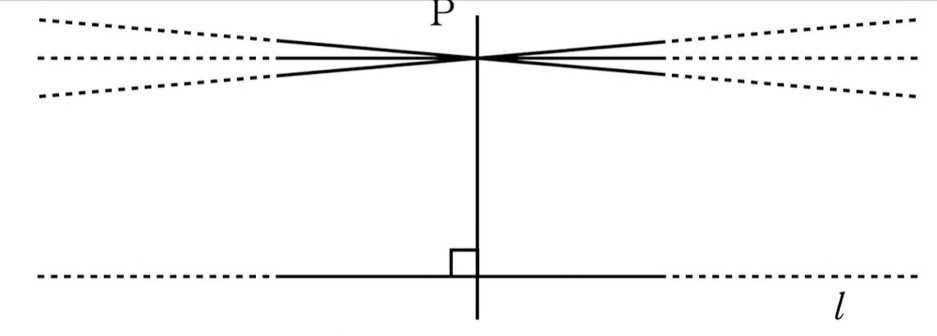
\includegraphics[width=0.7\textwidth]{images/axiom5.png}
    \caption{平行線と平行線にない点$p$を通る直線}
  \end{figure}
\end{frame}
\begin{frame}
  \frametitle{平行線公理への疑問}
  {\large 平行線公理は真理か}
  \begin{itemize}
  \item ほかの公準からの証明できないか
    \begin{itemize}
    \item アラビア世界ではハイタム(965-1039)やハイヤーミー(1048 – 1131)
    \item サッケーリ(1667ー1733), ルシャンドル(1752-1833)は独立に\\
      平行線公理がないと三角形の内角の和は二直角以下になると証明
    \end{itemize}
  \item \textcolor{highlight}{平行線公理を否定しても残りの公準と矛盾しない}
    \begin{itemize}
    \item ガウス(1777-1855)は平行線の公理は証明できないことを示唆する手紙を残す
    \item ロバチェフスキー(1792-1856)とボヤイ(1802-1860)が独立に平行線を二本以上ひけても矛盾しない非ユークリッド幾何学を発見
    \end{itemize}
  \end{itemize}
\end{frame}
\begin{frame}
  \frametitle{非ユークリッド空間の例}
  {\large 球面の大円は必ず交わる}
  \blfootnote{図は『はじめての構造主義』\supercite{structure}より}
  \begin{figure}
    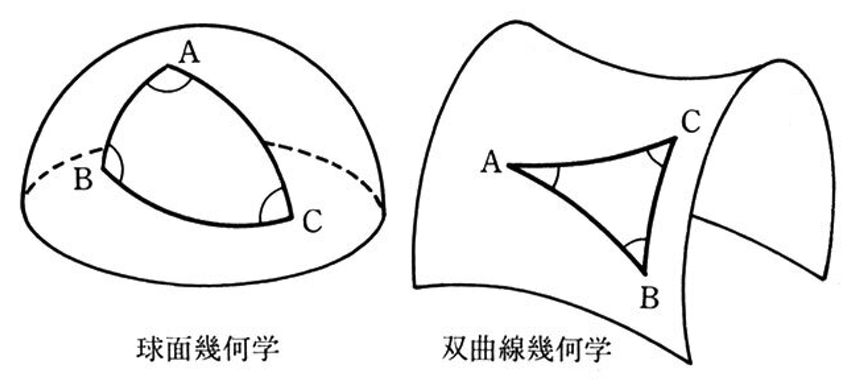
\includegraphics[width=0.5\textwidth]{images/non-euclid.png}
    \caption{非ユークリッド空間の例}
  \end{figure}
  \begin{itemize}
  \item 大円は中心を通る球の切断面
  \item 大円はユークリッド幾何学の直線にあたる
  \end{itemize}
\end{frame}
\section{素朴な集合論}
\begin{frame}
  \frametitle{非ユークリッド幾何学の影響}
  {\large 正しさは仮定した公理から作りだすもの}
  \begin{itemize}
  \item 空間を含む数学の対象は公理から構築するものになる
    \begin{itemize}
    \item ユークリッド幾何学を正しく感じるのは\\素朴な視覚の経験に合うから
    \item 原論の直線や平面の定義はあいまい
    \end{itemize}
  \item 数学の対象を定義する道具としてデデキントとカントールは\textcolor{highlight}{集合論}を確立
  \end{itemize}
\end{frame}
\begin{frame}
  \frametitle{ものの集まりで数学を考える}
  {\large 空集合だけで対象を定義できる}
  \par
  例
  \begin{enumerate}
  \item 空集合$\phi$を$\{x|x\neq x\}$とする
  \item $\phi$を$0$となづける
  \item 空集合1つからなる集合$\{\phi\}$を$1$となづける
  \item $\{0, 1\}$を$2$となづける
  \item $\vdots$
  \item $\{0, 1, 2, \cdots\}$を$\omega$となづける
  \item $\omega$の積集合$P(\omega)$を実数全体の集合にする
  \item $P(P(\omega))$を実数から実数への関数の集合にする
  \end{enumerate}
\end{frame}
\section{記号論理学}
\begin{frame}
  \frametitle{算術の基礎}
  {\large フレーゲは論理学を算術の基礎におこうとした}
  \begin{columns}
    \begin{column}{0.8\textwidth}
      \begin{itemize}
      \item 「概念記法」で\textcolor{highlight}{述語論理}を提案
      \item 「算術の基本法則」で概念記法と集合論による算術の公理と定理を提案
      \item ``On Sense and Reference''で語にはsenseとreferenceがあると提起
        \begin{itemize}
        \item 明けの明星と宵の明星のreferenceは金星
        \item 「金星は明けの明星である」と「金星は金星である」のsenseは違う
        \end{itemize}
      \end{itemize}
    \end{column}    
    \begin{column}{0.2\textwidth}
      \begin{figure}
        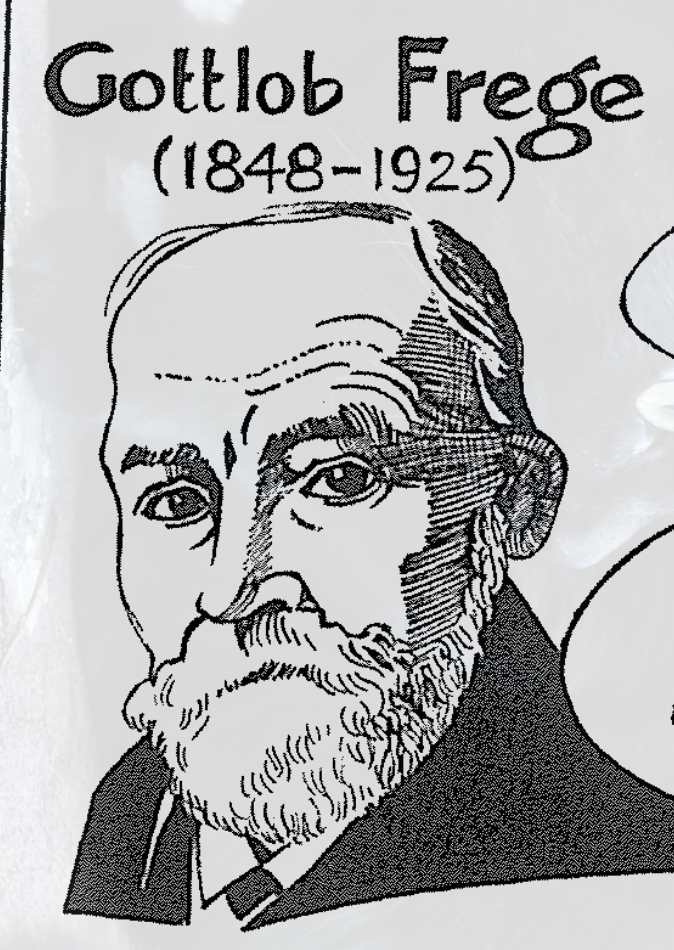
\includegraphics[width=1\textwidth]{images/frege.png}
      \end{figure}       
    \end{column} 
  \end{columns}
  \blfootnote{図はPhilosophy for beginners\supercite{philosophy-for-begginers}より}
\end{frame}
\begin{frame}
  \frametitle{思考を記号で計算する}
  {\large 推論を記号操作に還元する考えは17世紀以前からある}  
  \begin{columns}
    \begin{column}{0.55\textwidth}
      考案したもの
      \begin{itemize}
        \item 今日で使う微積分学の記法
        \item 二進数
        \item \textcolor{highlight}{characteristica universalis}
          \begin{itemize}
          \item 単語を構成するアルファベットのような思考の記号体系
          \item 代数的な記号操作で推論
          \end{itemize}
      \end{itemize}
    \end{column}    
    \begin{column}{0.4\textwidth}
      \begin{figure}
        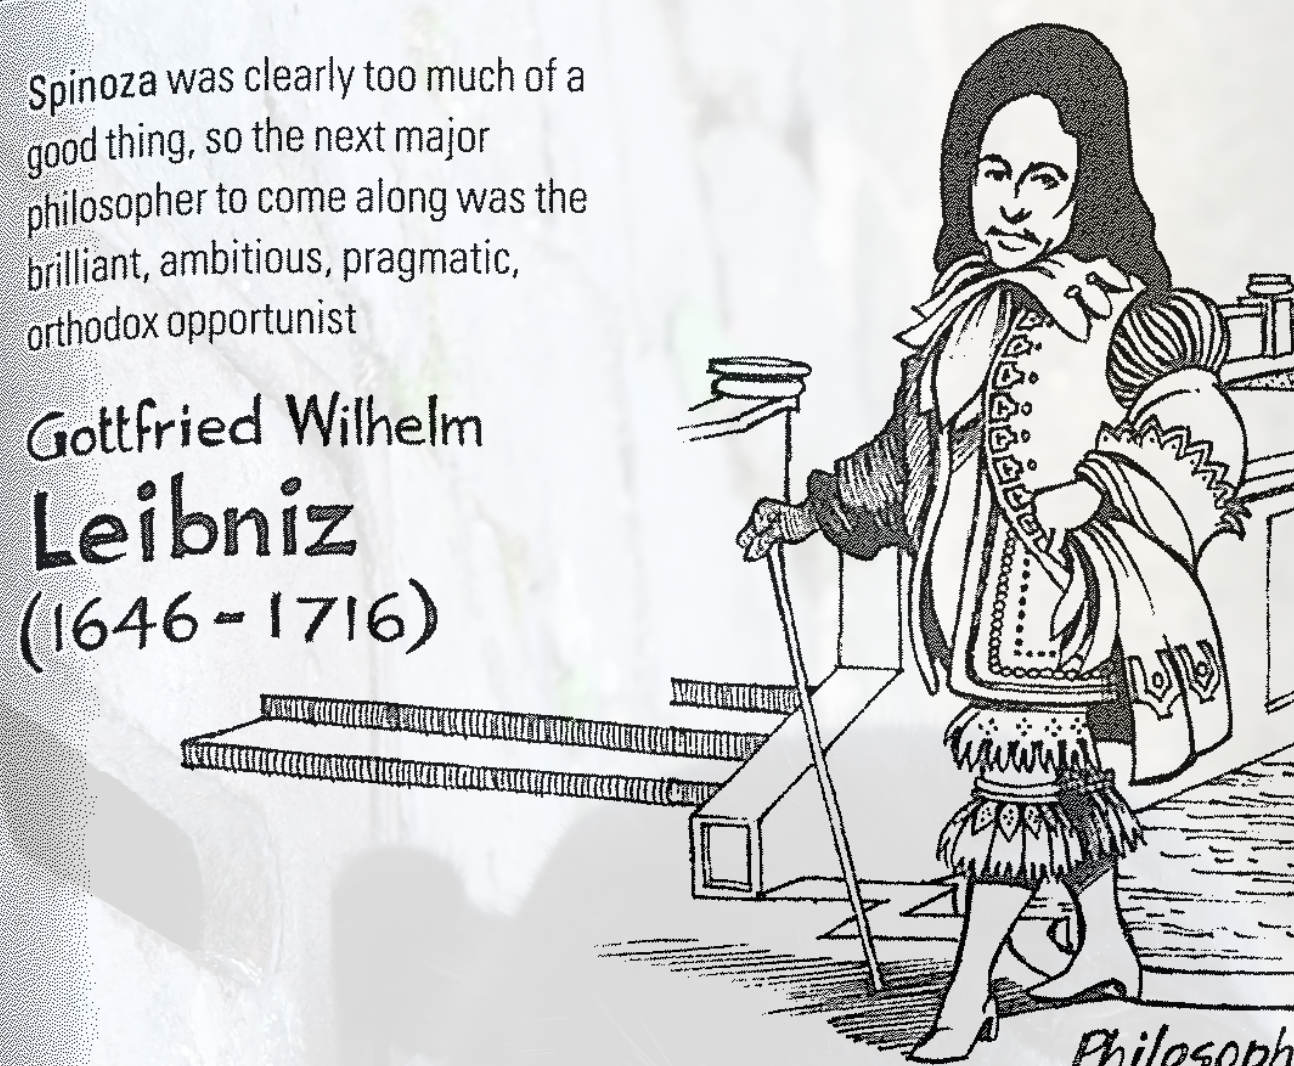
\includegraphics[width=0.7\linewidth]{images/leibniz.png}
        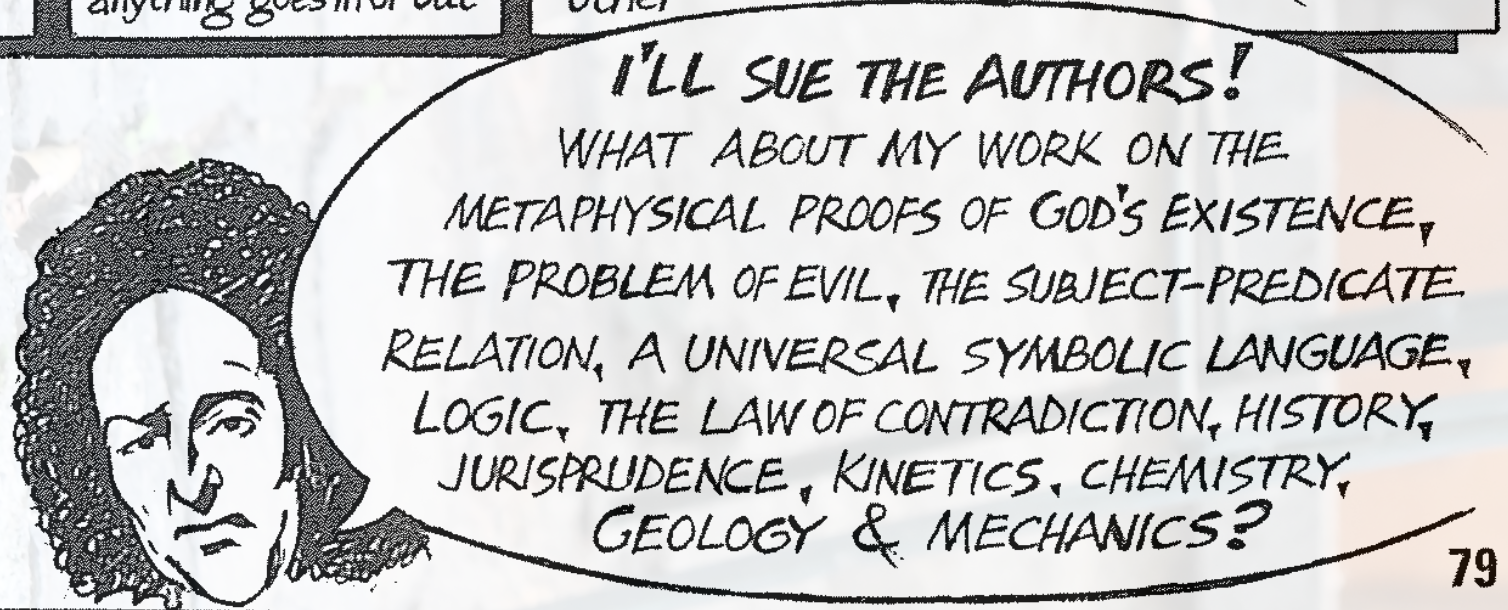
\includegraphics[width=0.7\linewidth]{images/universal.png}
      \end{figure}       
    \end{column} 
  \end{columns}
  \blfootnote{図はPhilosophy for beginners\supercite{philosophy-for-begginers}より}  
\end{frame}
\begin{frame}
  \frametitle{ブールの論理代数}
  {\large ブールは命題に出現する個体の集合を記号で表した}
  \begin{columns}
    \begin{column}{0.7\textwidth}
      \begin{center}
        THE LAWS OF THOUGHT\supercite{bool}より引用
        \begin{quotation}
          Let us then agree to represent \textcolor{highlight}{the class of individuals to which a particular name or description is applicable, by a single letter, as x}. If the name is “men,” for instance, let x represent “all men,”
        \end{quotation}
      \end{center}
    \end{column}    
    \begin{column}{0.2\textwidth}
      \begin{figure}
        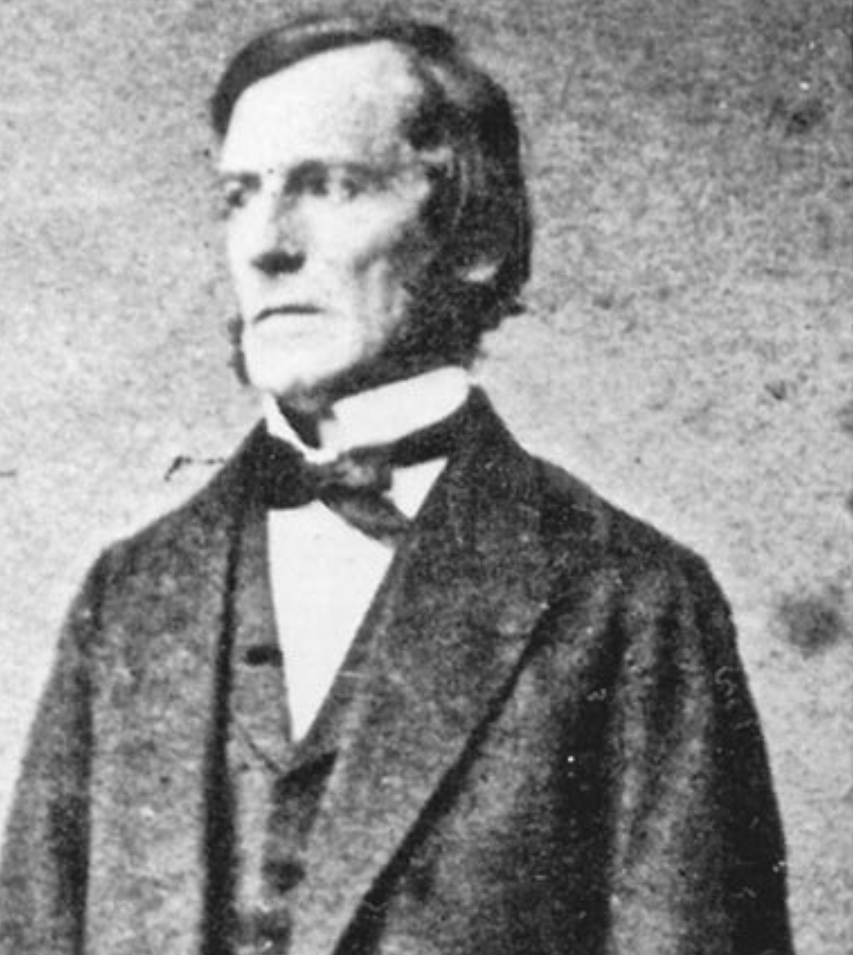
\includegraphics[width=1\textwidth]{images/bool.png}
      \end{figure}       
    \end{column} 
  \end{columns}
  \blfootnote{図は``The Universal Computer: The Road from Leibniz to Turing''より}
\end{frame}
\begin{frame}
  \frametitle{推論規則の例}
  {\large 命題論理は、命題と論理結合子からなる論理体系}
  \par
  推論規則
  \par
  \vspace{16pt}
  \AxiomC{$\varphi, \psi$}
  \RightLabel{(\wedge 導入)}
  \UnaryInfC{$\varphi\wedge\psi$}
  \DisplayProof
  \AxiomC{$\varphi\wedge\psi$}
  \RightLabel{(\vee 消去)}
  \UnaryInfC{$\varphi$}
  \DisplayProof
  \AxiomC{$\varphi\wedge\psi$}
  \RightLabel{(\vee 消去)}
  \UnaryInfC{$\psi$}
  \DisplayProof
  \AxiomC{$[\varphi]$}
  \noLine
  \UnaryInfC{$\vdots$}
  \noLine
  \UnaryInfC{$\psi$}
  \RightLabel{(\rightarrow 導入)}  
  \UnaryInfC{$\varphi\rightarrow\psi$}
  \DisplayProof
  \AxiomC{$\varphi$}
  \AxiomC{$\varphi\rightarrow\psi$}
  \RightLabel{(\rightarrow 消去)}  
  \BinaryInfC{$\psi$}
  \DisplayProof
  \AxiomC{$\bot$}
  \RightLabel{($\bot$)}
  \UnaryInfC{$\varphi$}
  \DisplayProof
  \AxiomC{$[\neg\varphi]$}
  \noLine
  \UnaryInfC{$\vdots$}
  \noLine
  \UnaryInfC{$\bot$}
  \RightLabel{(背理法)}
  \UnaryInfC{$\varphi$}
  \DisplayProof
  \par
  $\varphi,$, $\psi$は真偽値をとる命題。
\end{frame}
\begin{frame}
  \frametitle{概念記法}
  {\large フレーゲは述語による言明を形式化した}
  \begin{itemize}
  \item 「$\varphi$が〜である」という言明を引数$\varphi$を真偽値に写像する述語$P(\varphi)$をとして命題論理に加える
  \item \textcolor{highlight}{「任意の$\phi$について」という普遍量化子$\forall$と、「ある$x$について」という存在量化子$\exists$も加える}
  \item たとえば「家にいるペットは犬か猫だ」という命題は$\forall x. P(x) \rightarrow D(x)\vee C(x)$のように表せる
  \item 複雑な命題を単純な命題の組合せで表現しやすくなる
  \end{itemize} 
\end{frame}
\begin{frame}
  \frametitle{ラッセルのパラドクス}
  {\large \textcolor{highlight}{集合の集合}を考えると矛盾がおきる}
  \begin{enumerate}
  \item 自分自身を元にもたない集合すべての集合を\\$R=\{x|x\notin x \}$とする
  \item $R$が自分を元にもたない集合とすると定義から\\$R$は$R$の元になる
  \item $R$が自分を元にもつ集合とすると定義から\\$R$は$R$の元ではない
  \end{enumerate}  
\end{frame}
\begin{frame}
  \frametitle{「算術の基本法則」でのラッセルのパラドクス}
  {\large 原因は公理V: \textcolor{highlight}{$\epsilon P=\epsilon Q \equiv \forall x [P(x)\equiv Q(x)]$}}
  \begin{itemize}
  \item 公理Vは述語の同一である条件
  \item $\epsilon P$は述語$P$を充足する集合 
    \begin{enumerate}
    \item $R$を述語論理で$\exists P[x=\epsilon P\wedge \neg P(x)]$と表せる
    \item $x$を$\epsilon R$とすると$R(\epsilon R)\equiv\neg R(\epsilon R)$となる
    \end{enumerate}
  \item 型理論のはじまりは、述語論理の述語は述語をとれない規則のような階層構造でラッセルがパラドクスの解消を試みたこと
  \end{itemize}
\end{frame}
\begin{frame}[allowframebreaks,t]
  \frametitle{参考資料}
  \printbibliography
  \nocite{*}
\end{frame}

\end{document}
以上の内容を英訳してください。


Certainly! Here's the translation of the provided Beamer LaTeX document content into English:

```latex
\documentclass[unicode, 14pt, aspectratio=169]{beamer}
\usepackage{bussproofs}
\usetheme{titech}
\addbibresource{main.bib}
 \date{\number\year 年\number\month 月\number\day 日}
\title{The Origins of Type Theory}
\author{\texttt{ryotaro612}}

\newcommand\blfootnote[1]{%
  \begingroup
  \renewcommand\thefootnote{}\footnote{#1}%
  \addtocounter{footnote}{-1}%
  \endgroup
}

\begin{document}
\begin{frame}[noframenumbering, plain]
\titlepage
\end{frame}
\section{Introduction}
\begin{frame}
  \frametitle{Purpose of the Material}
  {\large Introduction to Fields Related to Type Theory}
  \par
  \vspace{16pt}
  Fields Related to the Reference Material
  \begin{itemize}
  \item Logic
  \item Set Theory
  \item Semiotics
  \item Structuralism
  \item Philosophy, especially Analytical Philosophy
  \end{itemize}
\end{frame}
\section{Geometry}
\begin{frame}
  \frametitle{Geometry Developed in Greece}
  {\large Geometric knowledge is a collection of \textcolor{highlight}{proofs}\footnote{Constructs were sometimes considered as proofs. The Greek word for “to prove” (deiknumi) also means “to show.” The origin of the word “demonstration.”} of theorems.}
\begin{columns}
  \begin{column}{0.25\textwidth}
    \begin{center}
      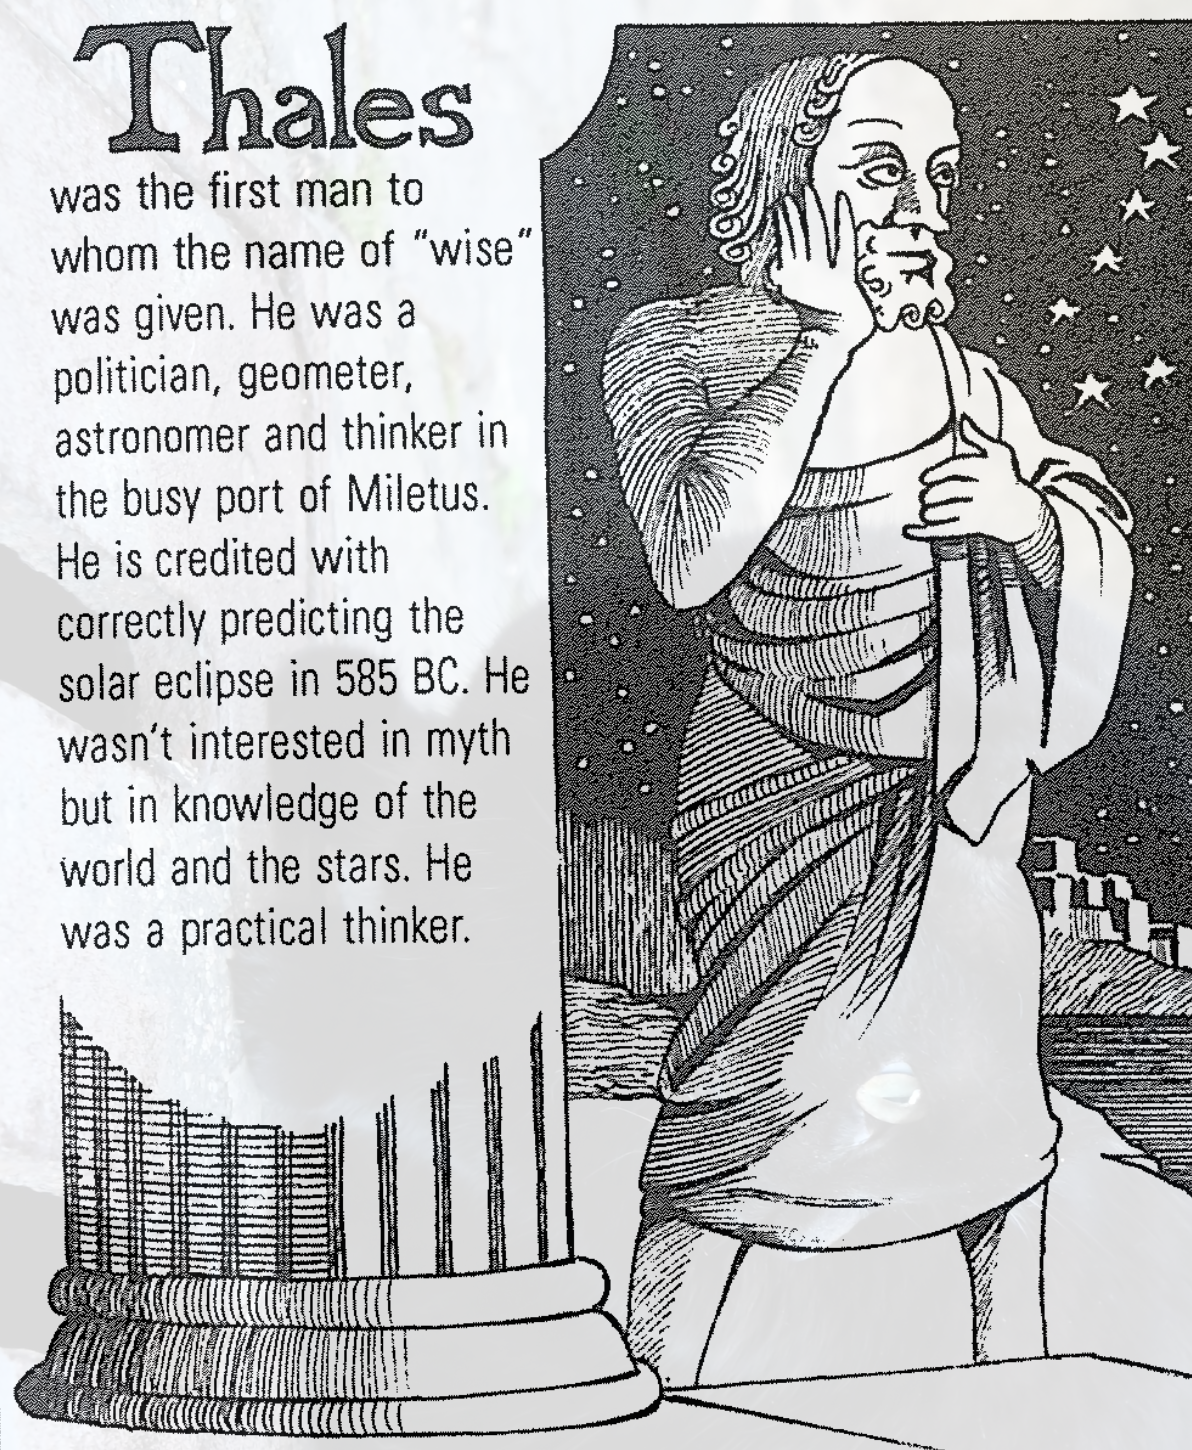
\includegraphics[width=0.7\textwidth]{images/thales.png}
    \end{center}
  \end{column}
  \begin{column}{0.25\textwidth}
    \begin{center}
      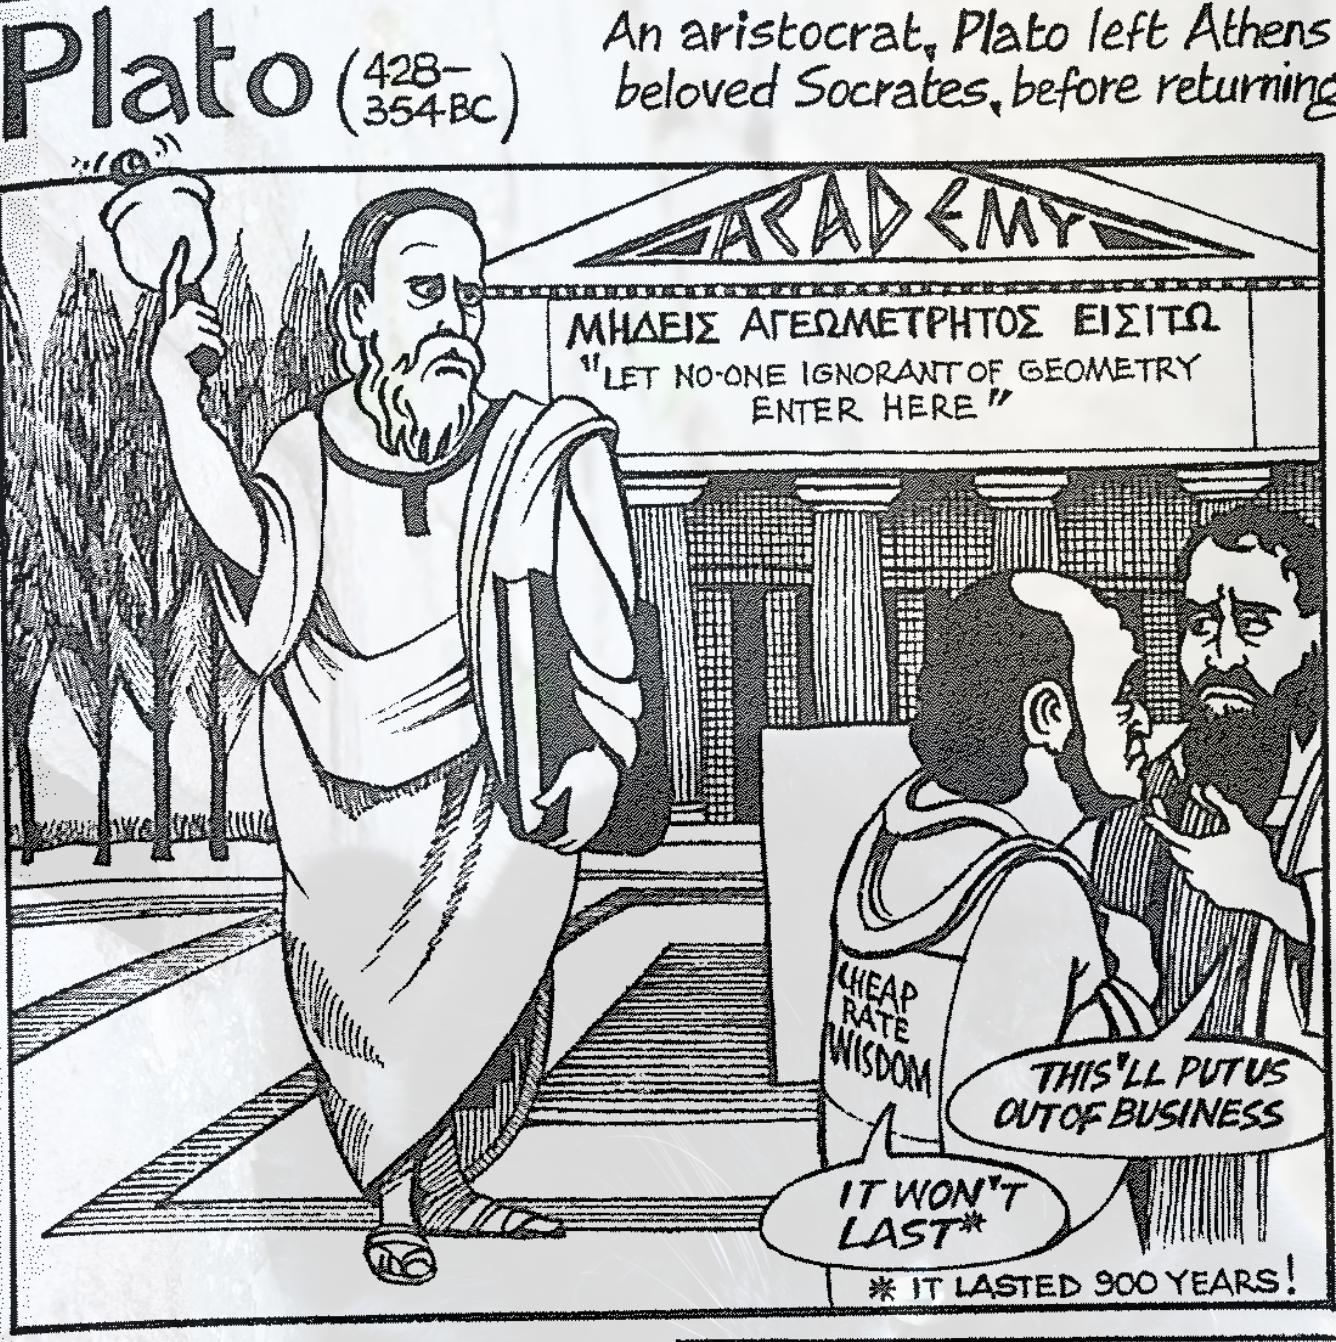
\includegraphics[width=0.7\textwidth]{images/plato.png}
    \end{center}
  \end{column}
  \begin{column}{0.25\textwidth}
    \begin{center}
      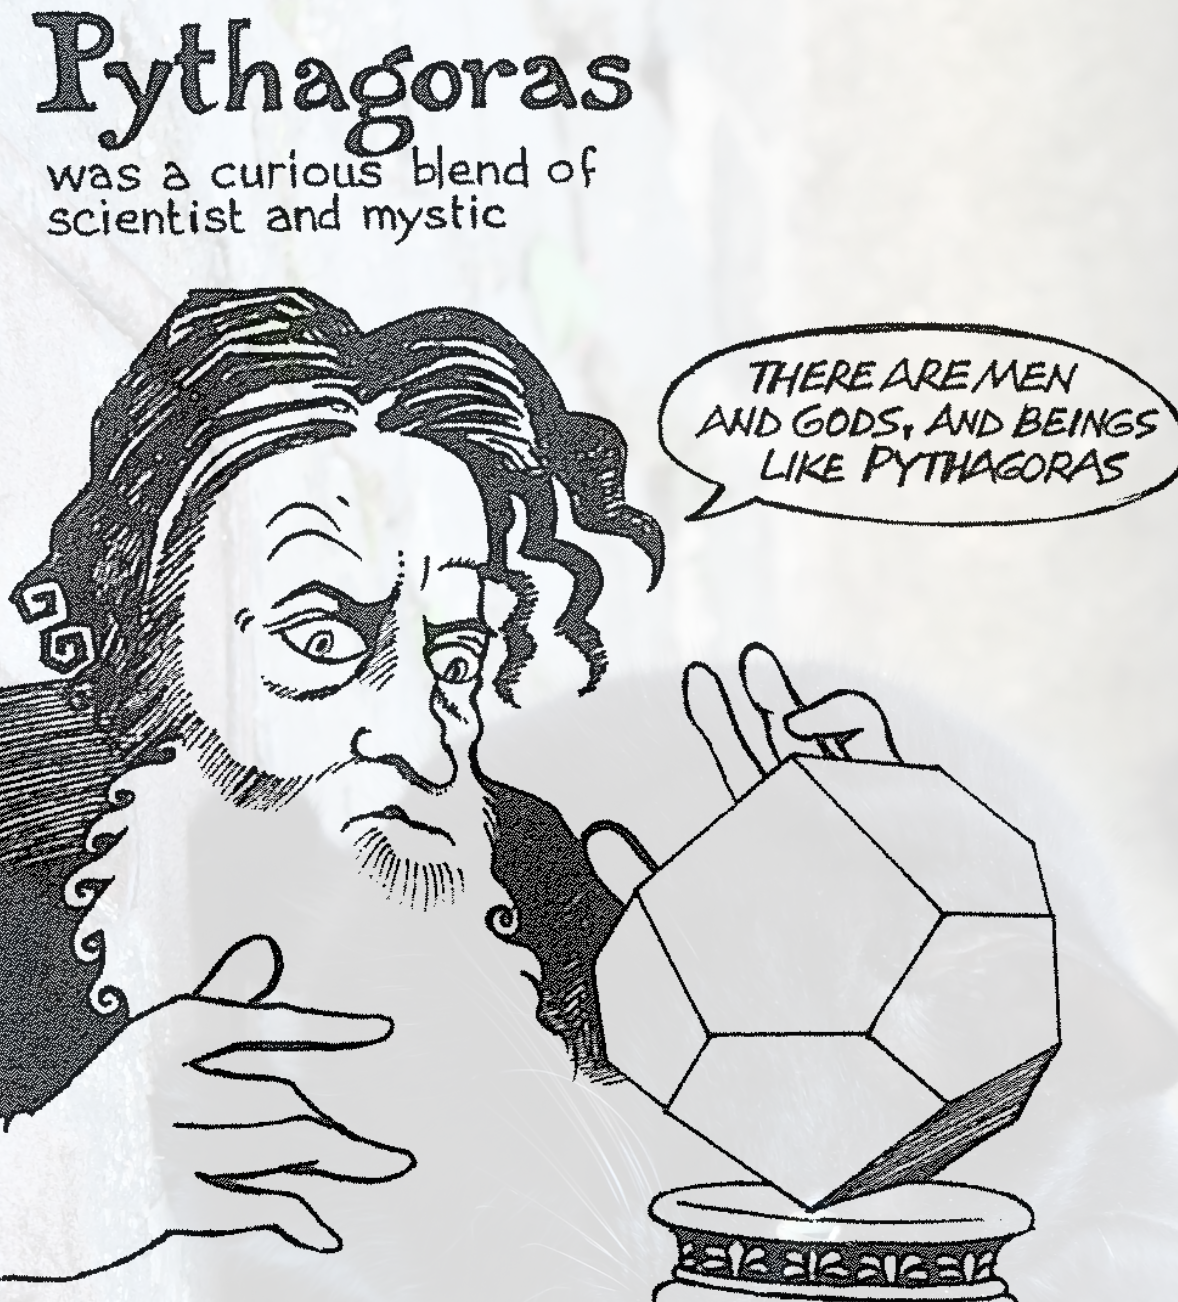
\includegraphics[width=0.7\textwidth]{images/pythagoras.png}
    \end{center}
  \end{column}
  \begin{column}{0.25\textwidth}
    \begin{center}
      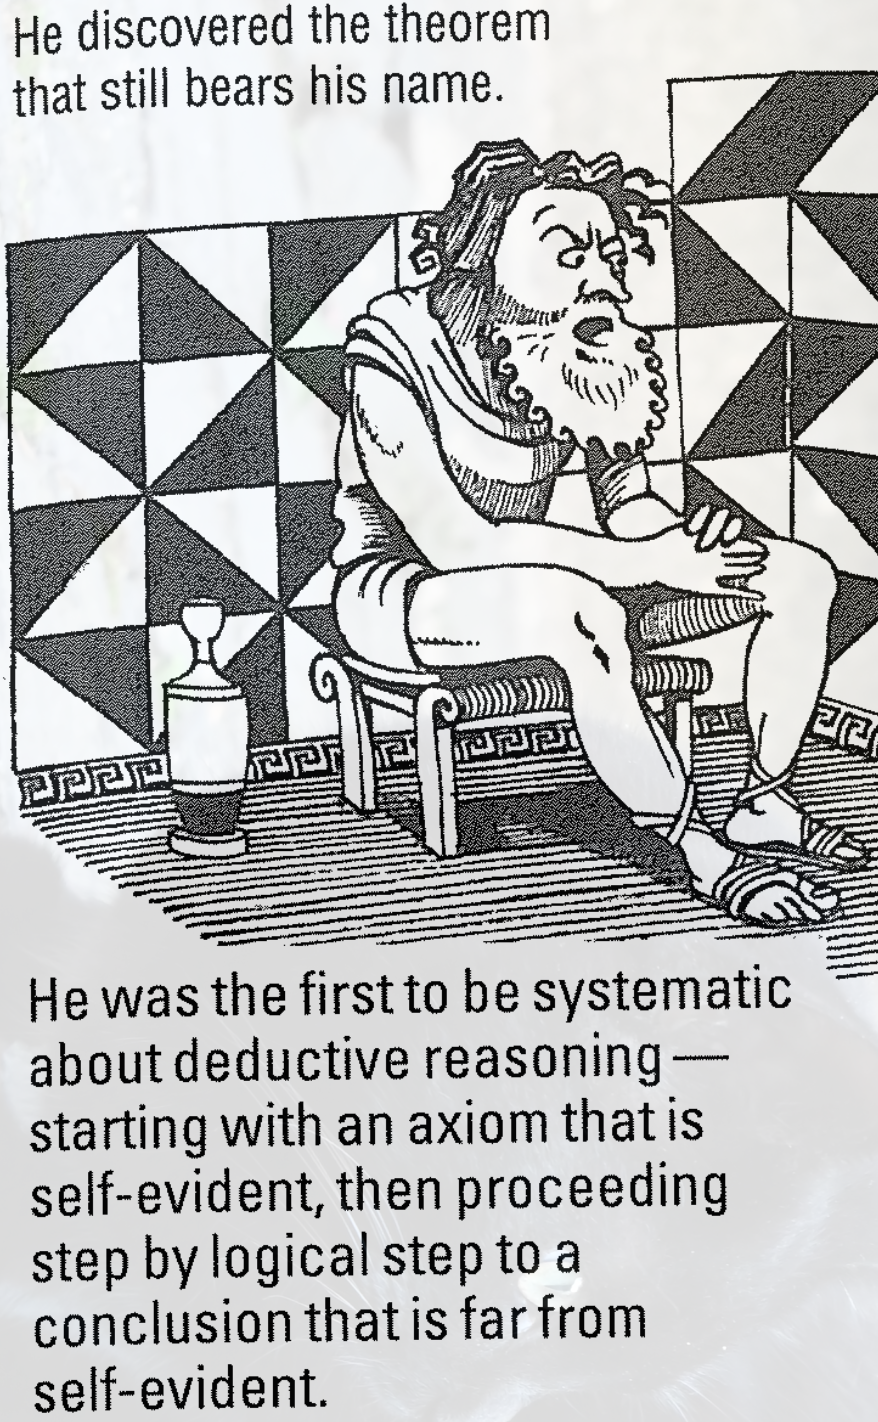
\includegraphics[width=0.7\textwidth]{images/pythagoras2.png}
    \end{center}
  \end{column}  
\end{columns}
\blfootnote{Figures from Philosophy for beginners\supercite{philosophy-for-begginers}} 
\end{frame}
\begin{frame}
  \frametitle{Euclid's Elements}
  {\large Geometry was organized into definitions, axioms, postulates\footnote{Axioms are premises for general entities like quantities, postulates are premises for geometric entities}, propositions, and proofs.}
  \par
  \vspace{16pt}
  Examples
  \begin{description}
  \item[Definition 1] A point is that which has no part
  \item[Definition 2] A line is breadthless length
  \item[Definition 3] A surface is that which has length and breadth only
  \item[Axiom 5] \textcolor{highlight}{The whole is greater than the part}
  \item[Proposition 5] The angles at the base of an isosceles triangle are equal to one another
  \end{description}
\end{frame}
\begin{frame}
  \frametitle{Five Postulates}
  {\large The fifth postulate is complex}
  \par
  \vspace{16pt}  
  \begin{enumerate}
  \item To draw a straight line from any point to any point
  \item To produce a finite straight line continuously in a straight line
  \item To describe a circle with any center and distance
  \item That all right angles are equal to one another
  \item \textcolor{highlight}{If a straight line falls on two straight lines in such a manner that the interior angles on the same side are together less than two right angles, the two straight lines, if produced indefinitely, meet on that side on which the angles are less than the two right angles.}
  \end{enumerate}
\end{frame}
\begin{frame}[t]
  \frametitle{The Fifth Postulate is also known as the Parallel Postulate}
  {\large Paraphrasing the fifth postulate: For any straight line and any point not on it, there exists exactly \textcolor{highlight}{one straight line parallel to the given one} through the point.}
  \blfootnote{Figure from "History of Mathematics in the World"\supercite{suugaku-no-sekaishi}}
  \begin{figure}
    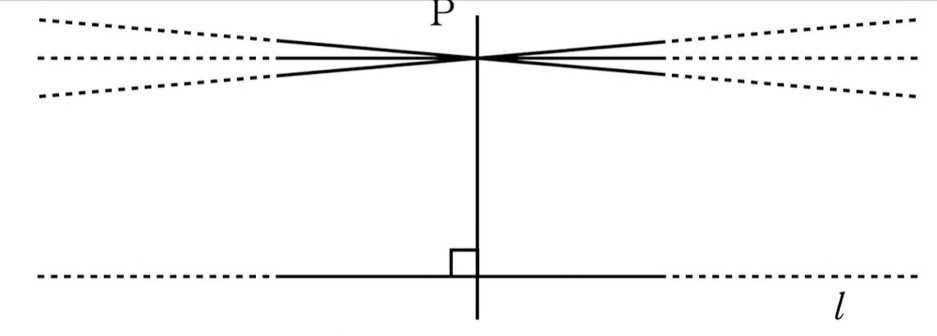
\includegraphics[width=0.7\textwidth]{images/axiom5.png}
    \caption{A parallel line passing through a point $p$ not on the given line}
  \end{figure}
\end{frame}
\begin{frame}
  \frametitle{Questioning the Parallel Postulate}
  {\large Is the parallel postulate a truth?}
  \begin{itemize}
  \item Can it be proven from the other postulates?
    \begin{itemize}
    \item In the Arab world, Alhazen (965-1039) and Khayyam (1048–1131) questioned it.
    \item Saccheri (1667–1733) and Legendre (1752–1833) independently showed that without the parallel postulate, the sum of the angles in a triangle is less than or equal to two right angles.
    \end{itemize}
  \item \textcolor{highlight}{Denying the parallel postulate does not contradict the remaining postulates.}
    \begin{itemize}
    \item Gauss (1777-1855) suggested in letters that the parallel postulate cannot be proved.
    \item Lobachevsky (1792-1856) and Bolyai (1802-1860) independently discovered non-Euclidean geometry where more than one line can be drawn parallel to a given line without contradiction.
    \end{itemize}
  \end{itemize}
\end{frame}
\begin{frame}
  \frametitle{Examples of Non-Euclidean Spaces}
  {\large Great circles on a sphere must intersect.}
  \blfootnote{Figure from "An Introduction to Structuralism"\supercite{structure}}
  \begin{figure}
    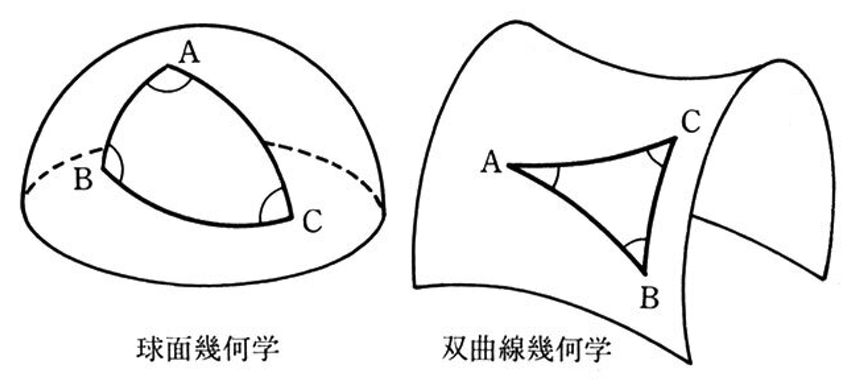
\includegraphics[width=0.5\textwidth]{images/non-euclid.png}
    \caption{Example of a non-Euclidean space}
  \end{figure}
  \begin{itemize}
  \item Great circles are cross-sections of spheres passing through the center.
  \item Great circles correspond to straight lines in Euclidean geometry.
  \end{itemize}
\end{frame}
\section{Naive Set Theory}
\begin{frame}
  \frametitle{Impact of Non-Euclidean Geometry}
  {\large Correctness is based on the axioms assumed.}
  \begin{itemize}
  \item Mathematical objects, including space, are constructed from axioms.
    \begin{itemize}
    \item Euclidean geometry feels correct because it aligns with naive visual experience.
    \item Definitions of lines and planes in "Elements" are vague.
    \end{itemize}
  \item \textcolor{highlight}{Set theory} was established by Dedekind and Cantor as a tool to define mathematical objects.
  \end{itemize}
\end{frame}
\begin{frame}
  \frametitle{Thinking of Mathematics as Collections of Objects}
  {\large Everything can be defined using the empty set.}
  \par
  Example
  \begin{enumerate}
  \item Define the empty set $\phi$ as $\{x|x\neq x\}$.
  \item Name $\phi$ as $0$.
  \item The set containing a single empty set $\{\phi\}$ is named $1$.
  \item Name $\{0, 1\}$ as $2$.
  \item $\vdots$
  \item Name $\{0, 1, 2, \cdots\}$ as $\omega$.
  \item Make the power set of $\omega$, $P(\omega)$, the set of real numbers.
  \item Make $P(P(\omega))$ the set of functions from real numbers to real numbers.
  \end{enumerate}
\end{frame}
\section{Symbolic Logic}
\begin{frame}
  \frametitle{Foundation of Arithmetic}
  {\large Frege attempted to base arithmetic on logic.}
  \begin{columns}
    \begin{column}{0.8\textwidth}
      \begin{itemize}
      \item Proposed \textcolor{highlight}{predicate logic} in "Conceptual Notation."
      \item Suggested axioms and theorems of arithmetic via conceptual notation and set theory in "The Basic Laws of Arithmetic."
      \item In "On Sense and Reference," posited that words have both a sense and a reference.
        \begin{itemize}
        \item The reference of the "morning star" and "evening star" is Venus.
        \item The sense of "Venus is the morning star" differs from "Venus is Venus."
        \end{itemize}
      \end{itemize}
    \end{column}    
    \begin{column}{0.2\textwidth}
      \begin{figure}
        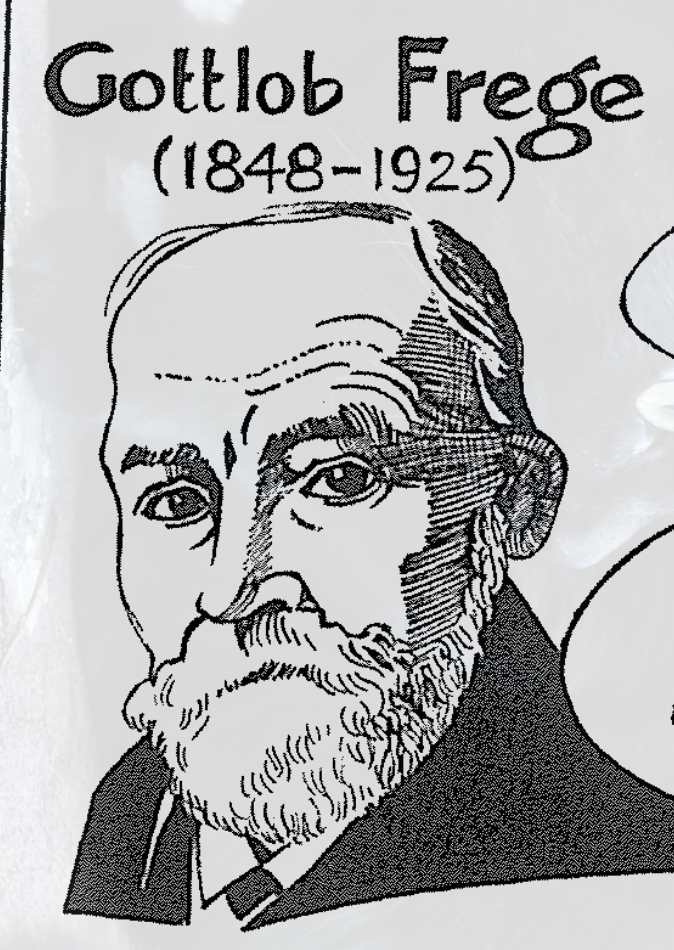
\includegraphics[width=1\textwidth]{images/frege.png}
      \end{figure}       
    \end{column} 
  \end{columns}
  \blfootnote{Figures from Philosophy for beginners\supercite{philosophy-for-begginers}}
\end{frame}
\begin{frame}
  \frametitle{Formalizing Thought with Symbols}
  {\large The idea to reduce inference to symbolic manipulation has existed since the 17th century or earlier.}  
  \begin{columns}
    \begin{column}{0.55\textwidth}
      Those who devised it:
      \begin{itemize}
        \item Notation for calculus used today
        \item The binary number system
        \item \textcolor{highlight}{characteristica universalis}
          \begin{itemize}
          \item A set of symbols for thought analogous to the alphabet for language.
          \item Reasoning is done through algebraic operations with symbols.
          \end{itemize}
      \end{itemize}
    \end{column}    
    \begin{column}{0.4\textwidth}
      \begin{figure}
        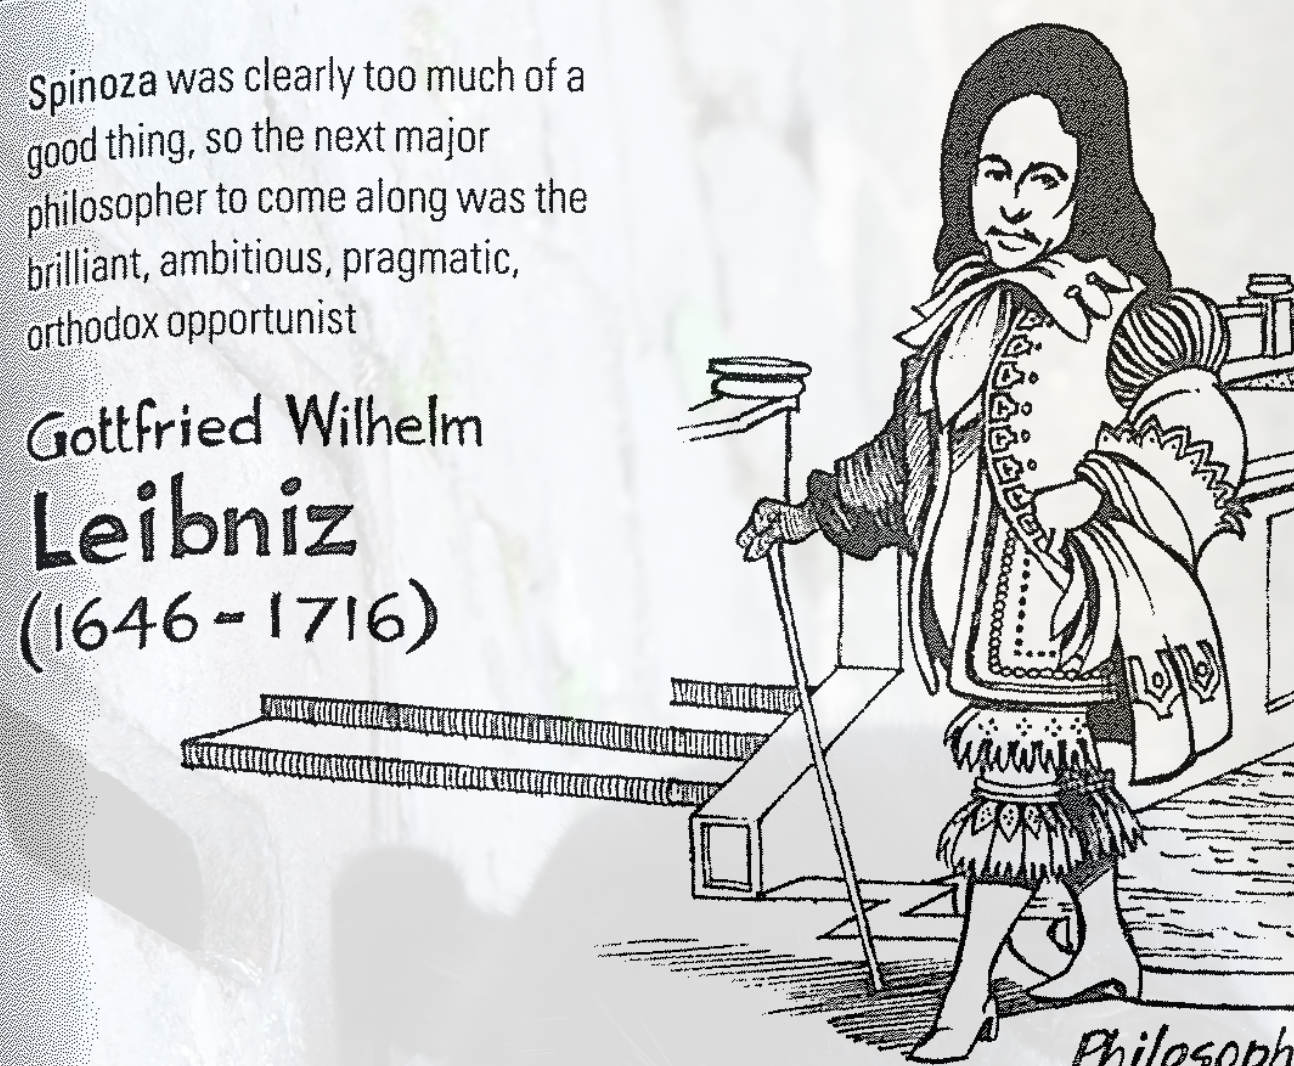
\includegraphics[width=0.7\linewidth]{images/leibniz.png}
        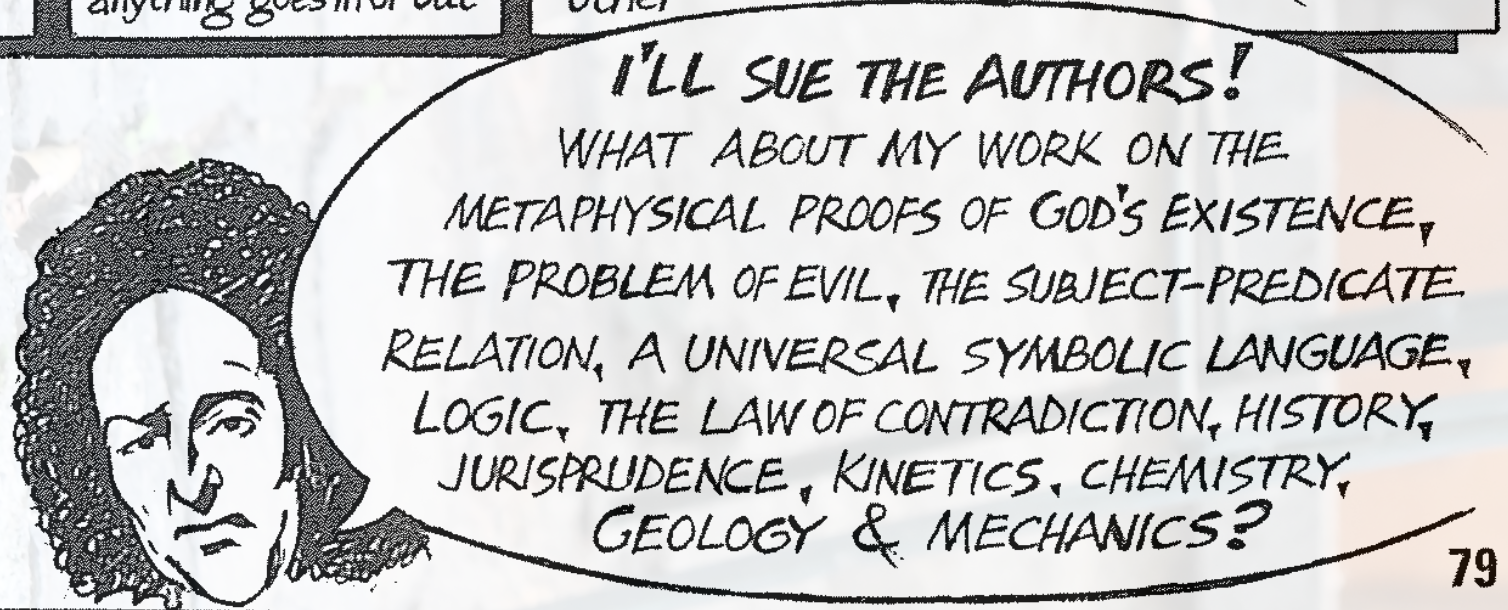
\includegraphics[width=0.7\linewidth]{images/universal.png}
      \end{figure}       
    \end{column} 
  \end{columns}
  \blfootnote{Figures from Philosophy for beginners\supercite{philosophy-for-begginers}}  
\end{frame}
\begin{frame}
  \frametitle{Boole's Logical Algebra}
  {\large Boole represented the sets of individuals appearing in propositions using symbols.}
  \begin{columns}
    \begin{column}{0.7\textwidth}
      \begin{center}
        Quotation from "The Laws of Thought"\supercite{bool}:
        \begin{quotation}
          Let us then agree to represent \textcolor{highlight}{the class of individuals to which a particular name or description is applicable, by a single letter, as x}. If the name is “men,” for instance, let x represent “all men,”
        \end{quotation}
      \end{center}
    \end{column}    
    \begin{column}{0.2\textwidth}
      \begin{figure}
        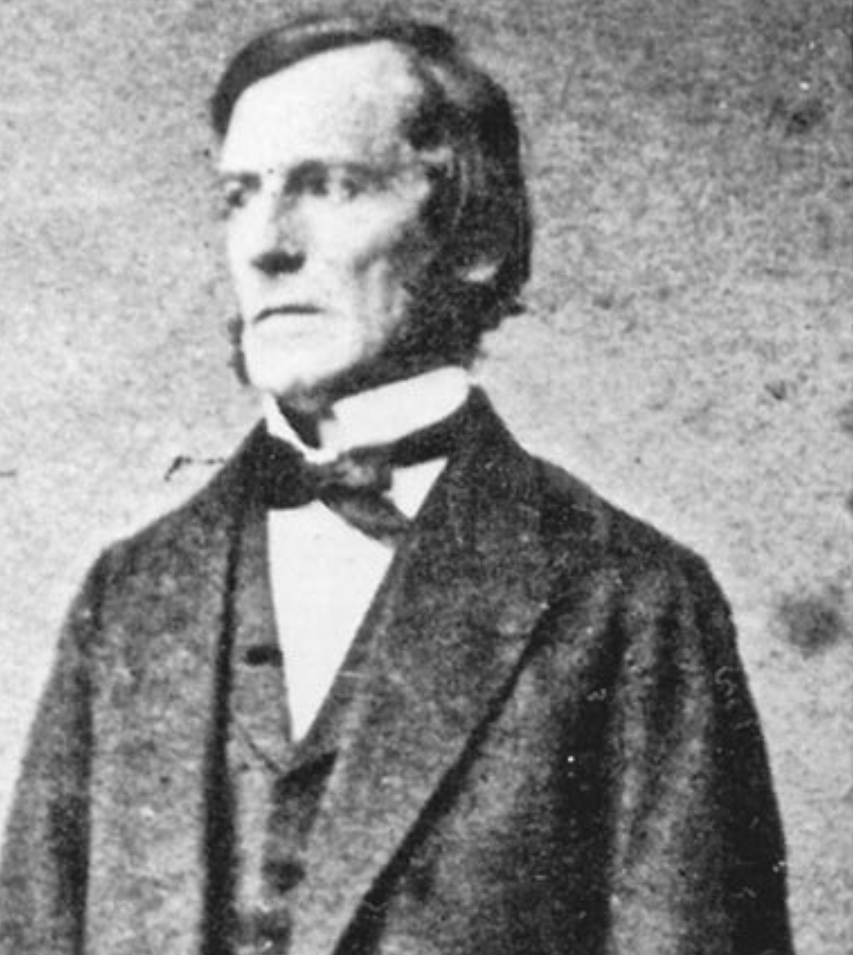
\includegraphics[width=1\textwidth]{images/bool.png}
      \end{figure}       
    \end{column} 
  \end{columns}
  \blfootnote{Figures from "The Universal Computer: The Road from Leibniz to Turing"}
\end{frame}
\begin{frame}
  \frametitle{Examples of Inference Rules}
  {\large Propositional logic is a logical system composed of propositions and logical connectives.}
  \par
  Inference rules:
  \par
  \vspace{16pt}
  \AxiomC{$\varphi, \psi$}
  \RightLabel{(\wedge Introduction)}
  \UnaryInfC{$\varphi\wedge\psi$}
  \DisplayProof
  \AxiomC{$\varphi\wedge\psi$}
  \RightLabel{(\vee Elimination)}
  \UnaryInfC{$\varphi$}
  \DisplayProof
  \AxiomC{$\varphi\wedge\psi$}
  \RightLabel{(\vee Elimination)}
  \UnaryInfC{$\psi$}
  \DisplayProof
  \AxiomC{$[\varphi]$}
  \noLine
  \UnaryInfC{$\vdots$}
  \noLine
  \UnaryInfC{$\psi$}
  \RightLabel{(\rightarrow Introduction)}  
  \UnaryInfC{$\varphi\rightarrow\psi$}
  \DisplayProof
  \AxiomC{$\varphi$}
  \AxiomC{$\varphi\rightarrow\psi$}
  \RightLabel{(\rightarrow Elimination)}  
  \BinaryInfC{$\psi$}
  \DisplayProof
  \AxiomC{$\bot$}
  \RightLabel{($\bot$)}
  \UnaryInfC{$\varphi$}
  \DisplayProof
  \AxiomC{$[\neg\varphi]$}
  \noLine
  \UnaryInfC{$\vdots$}
  \noLine
  \UnaryInfC{$\bot$}
  \RightLabel{(Reductio ad Absurdum)}
  \UnaryInfC{$\varphi$}
  \DisplayProof
  \par
  $\varphi$, and $\psi$ are propositions that can take truth values.
\end{frame}
\begin{frame}
  \frametitle{Conceptual Notation}
  {\large Frege formalized statements with predicates.}
  \begin{itemize}
  \item Statements like “$\varphi$ is ~” are represented by predicates $P(\varphi)$ that map argument $\varphi$ to truth values, added to propositional logic.
  \item \textcolor{highlight}{Also adds the universal quantifier $\forall$ for “for any $\phi$,” and the existential quantifier $\exists$ for “there exists $x$.”}
  \item For instance, the statement “Pets at home are either dogs or cats” is represented as $\forall x. P(x) \rightarrow D(x) \vee C(x)$.
  \item Complex propositions can be easily expressed as combinations of simpler ones.
  \end{itemize} 
\end{frame}
\begin{frame}
  \frametitle{Russell's Paradox}
  {\large A contradiction arises when considering \textcolor{highlight}{sets of sets}.}
  \begin{enumerate}
  \item Define the set $R$ of all sets that do not contain themselves as a member: $R = \{x | x \notin x \}$.
  \item If $R$ is a set that does not contain itself, then by definition, $R$ should be a member of $R$.
  \item If $R$ is a set that contains itself, then by definition, $R$ should not be a member of $R$.
  \end{enumerate}  
\end{frame}
\begin{frame}
  \frametitle{Russell's Paradox in "The Basic Laws of Arithmetic"}
  {\large The cause is Axiom V: \textcolor{highlight}{$\epsilon P = \epsilon Q \equiv \forall x [P(x) \equiv Q(x)]$.}}
  \begin{itemize}
  \item Axiom V is the condition for the identity of predicates.
  \item $\epsilon P$ is the set fulfilling predicate $P$. 
    \begin{enumerate}
    \item $R$ can be expressed using predicate logic as $\exists P [x = \epsilon P \wedge \neg P(x)]$.
    \item Substituting $x$ as $\epsilon R$, we obtain $R(\epsilon R) \equiv \neg R(\epsilon R)$.
    \end{enumerate}
  \item The beginning of type theory involved Russell's attempt to resolve the paradox by imposing a hierarchical structure, such as predicates of predicate logic not being able to take predicates.
  \end{itemize}
\end{frame}
\begin{frame}[allowframebreaks,t]
  \frametitle{References}
  \printbibliography
  \nocite{*}
\end{frame}

\end{document}
